\documentclass{article}
\usepackage{fullpage}

\usepackage{enumerate}
\usepackage{tabu}
\usepackage{setspace}
\usepackage{sectsty}
\usepackage{soul,xcolor}
\usepackage{titlesec}
\usepackage{fancyhdr}
\usepackage{color}
\usepackage{hyperref}
\usepackage[tocindentauto]{tocstyle}
\usepackage[final]{pdfpages}

\hypersetup{
    colorlinks=true,
    linkcolor= blue,
    filecolor=magenta,      
    urlcolor=cyan,
}

\title{The Unofficial, Semi-Comprehensive, Quintessential UC Davis Computer Science Major Handbook and FAQ}
\author{The Davis Computer Science Club}
\date{Version 0.0\\September 14, 2016}

\begin{document}

\begin{titlepage}
	\maketitle
\end{titlepage}

\newpage

\tableofcontents

\pagebreak

\singlespacing
\sectionfont{\Large}
\subsectionfont{\large}

\section {Version History of this Handbook}
\subsection*{Version 0.0}
September 14, 2016. First version of the handbook written.
\newpage
\section{Introduction and Disclaimer}
\hspace{0.5cm}I started writing this handbook with a few others because I saw a sore lack of resources for not just the UC Davis Computer Science community, but the tech community in general. More importantly, I knew that a lot of my peers, especially peers who weren't considered the stereotypical Computer Science student, had questions but were too scared to ask them due to fear of backlash and critique. \\

Like most CS students, I started CS without any Computer Science background and learned everything in this handbook the hard way. Hence, this handbook was written in mind with the audience being a complete newbie (aka a first year with no Computer Science knowledge at all) as a brief overview. \\

I don't know how helpful this handbook will be or if anyone's attempted anything like this before, but I thought I'd try my hand at sharing my knowledge with anyone who'd be interested. I don't claim to know everything and I'm sure those with more experience could add more nuance and details onto whatever modest amount I have here. If you're interested in adding more to this handbook, please submit a pull request to the Github repository where this is hosted. Please feel free to contact The Davis Computer Science Club with any questions! 
\subsection{How to Best Use This Handbook}
\hspace{0.5cm}There's a lot in this handbook! You don't have to read this handbook cover to cover, word by word (though I'd love it if you did!), but just read whatever sections you're interested in by going to the Contents page and clicking on any section you'd like to read. Any URL to another site is highlighted in \textcolor{cyan}{cyan blue}, and any links/hooks within the document are highlighted in \textcolor{blue}{plain blue}. 
\subsection{Disclaimer}\\
\hspace{0.5cm}This handbook only offers advice and resources given by few members of the UC Davis Computer Science Club -- it is by no means a strict guideline for one to follow or a guarantor of success and is not meant to serve as a replacement or substitute for advising by a counselor or adviser. If you have questions, this handbook is a place meant to start your research, not to complete it. While we do our best to make sure our information is accurate and updated, mistakes can be made either from human error or the handbook simply not being updated to match current changes-- please make sure to confirm all information with an adviser or through other resources.\\

If you have questions or comments, or would like to provide suggestions, please feel free to email one of the current officers here:
\nameref{sec:DCSC}. If you would like to add more to the handbook or fix a mistake, please feel free to submit a pull request to the repository where this handbook is hosted. Thank you! \\\\
\textbf{Written with love in LaTeX by:} \\
Stephanie Chang '17 \\ \\ 
\textbf{With contributions by:} \\
Alex Fu '17\\
David Lin '17\\
Christina Zhu '17\\
The Davis Computer Science Club\\

\newpage
\section {The Davis Computer Science Club}
\label{sec:DCSC}
\hspace{0.5cm}The Davis Computer Science club runs during the school-year and provides resources, workshops, and a community for the UC Davis Computer Science community. Here's a breakdown of the Davis Computer Science Club:\\

Besides the main board, we have three committees -- Tutoring, Pragmatic Programming, and Professional Development. Each committee is headed by a chair and their possible, respective co-chair. Our website and various pages can be found below: \\
\begin{center}
{\tabulinesep=1.2mm
\begin{tabu} {|p{3cm} |p{8cm}|}
\hline
\textbf{Link} & \textbf{Description} \\ 
\hline
\href{http://daviscsclub.org}{Website} & Our main page -- information about the Davis CS Club, its officers, committees, and various events are located here. \\
\hline
\href{https://www.facebook.com/groups/daviscsclub/}{Facebook Group} & Chat with other CS majors at UCD and find out about our events \\
\hline
\href{https://www.facebook.com/daviscsclub}{Facebook Page} & A little different from the Facebok group -- you can find photos and event information here.\\
\hline
\href{https://github.com/DavisCSClub}{Github} & Our study guides for upper division classes, class notes, meeting minutes, officer board, bylaws, and whatnot are all hosted here.\\
\hline
\end{tabu}}\\
\end{center}
\hspace{0.5cm} One of our old committees, the Game Development Committee, has branched off from the Davis Computer Science Club and has created their own club -- if interested, please check \href{https://www.facebook.com/groups/davisgamedev/}{here}.
\subsection {General Events}
\hspace{0.5cm}Here are the general events, workshops, and programs the Davis Computer Science Club holds either quarterly or yearly. Some events may or may not be included at the discretion of the current board whereas some events may be added. To keep updated, join our Facebook group or follow us on our Facebook page! 
\begin{itemize}
    \item Bit/Byte Mentorship Program
    \item Gender Diversity in Tech 
    \item Courses Preview
    \item Socials
    \item DCSC End-Of-Year Banquet
    \item Elections
    \item T-shirt contest
\end{itemize}
\subsection{Tutoring Committee}
\hspace{0.5cm} The Tutoring Committee serves the Davis Computer Science community by training and providing volunteer tutors for Computer Science (ECS) courses at UC Davis. \\

Tutors are typically located in Kemper Basement during their signed up hours, but are possibly available upon request. The Tutoring Committee also holds review sessions for lower division ECS courses and a select few upper division courses depending on the availability of the tutors who are able to lead the review sessions. \\

Tutors are able to receive undergraduate ECS credit with a certain amount of hours. To become a tutor, contact the current Tutoring Committee chair(s) or the Davis Computer Science club. \\

To find a tutor, please check \href{https://daviscsclub.org/tutoring/athena}{athena} for available tutors during the week, or Kemper 75 or Kemper 77 during CSIF hours on weekdays. 
\subsection{Pragmatic Programming Committee}
\hspace{0.5cm} Pragmatic Programming tends to lead workshops on various skills, tools, languages, frameworks, and so on forth in tech and Computer Science. They may be spread out in a series of weeks. Past workshops include, but are not limited to: 
\begin{itemize}
    \item iOS and Android Development I, II, III, IV
    \item Web Development
    \item Javascript
    \item Git
    \item Building Your Own Application 
    \item Optimization 
\end{itemize}

And so on forth. If interested in participating in events, please check out the Facebook group or page to see if any events are running! If you're interested in helping out, please get in contact with our current Pragmatic Programming chair(s).
\subsection{Professional Development Committee}
\hspace{0.5cm}The Professional Development provides a series of workshops and events to help students with advancing their careers. Past events have included, but are not limited to: 
\begin{itemize}
    \item Mock Interviews
    \item Resume Workshops
    \item Negotiating Offers
    \item Alumni Talks 
    \item Professor Chats with Professor Rogaway, Professor Gysel, Professor Filikov, and so on forth
\end{itemize}

And so on forth. If interested in participating in events, please check out the Facebook group or page to see if any events are running! If you're interested in helping out, please get in contact with our current Professional Development chair(s).
\subsection{Web Development Committee}
\hspace{0.5cm} Web Development is in charge of our website, daviscsclub.org. They design, host, and code up the website and keep it updated. There are no particular events that the Web Development committee hosts, but people are welcome to attend and help out the committee and website and get acquainted with the code that is involved with our website! If you're intersted, please contact our Web Development chair(s).
\subsection {How to Get Involved}
\hspace{0.5cm} Attend workshops, events, and officer meetings, join our Facebook group and follow our Facebook page! Become a mentor a mentee for the Bit/Byte mentorship program, and volunteer at our events! We need volunteers to help out with any large event we plan, such as Gender Diversity in Tech and our DCSC End-Of-Year Banquet. If interested in helping out or attending, message us on our Facebook page. :)

\subsection{Officer Board 2016-2017}
\label{sec:officers}
\hspace{0.5cm} You can find a description of the officer board in our Bylaws  \href{https://github.com/DavisCSClub/Bylaws/blob/master/bylaws.pdf}{here}. Our weekly officer meetings are open to the public -- if interested in attending, please message the Davis Computer Science Club on our Facebook page as they are subject to change weekly depending on the availability of the board.
\\\begin{center}
\textbf{Core Body}
\end{center}
\begin{center}
\begin{tabular} {|c|c|c|}
\hline
\textbf{Title} & \textbf{Officer} & \textbf{Contact} \\
\hline
President & Pooja Rajikumar & prajkumar@ucdavis.edu \\
\hline
Internal Vice President & Stephanie Chang & ischang@ucdavis.edu \\
\hline
External Vice President & Ariel Shin & arishin@ucdavis.edu \\
\hline
Treasurer & Sam Tsoi & sgtsoi@ucdavis.edu\\
\hline
Secretary & Trevor Glynn & tfglynn@ucdavis.edu \\
\hline
Events Coordinator & Sravya Divakarla  & sdivakarla@ucdavis.edu\\
\hline
Marketing Director & Prajakta Surve & prsurve@ucdavis.edu\\
\hline
\end{tabular} 
\end{center}
\begin{center}
\textbf{Committees}
\end{center}
\begin{center}
\begin{tabular} {|c|c|c|}
\hline
\textbf{Committee} & \textbf{Chair} & \textbf{Contact} \\
\hline
Tutoring & Alex Fu & aafu@ucdavis.edu \\
\hline
Pragmatic Programming & Pranav Gupta & phgupta@ucdavis.edu \\
\hline
Professional Development & Zain Budhwani & zbud@ucdavis.edu\\
\hline
Web Development & Teresa Liu & stiliu@ucdavis.edu \\
\hline
\end{tabular}
\end{center}
\subsection{FAQ}
\begin{enumerate}
    \item \textbf{Are there any requirements to becoming a member of the Davis Computer Science Club?}
    \begin{itemize}
        Nope! Regardless of major or age, anyone is free to participate in our events and workshops. We only ask that you be polite and respectful to everyone else. 
    \end{itemize}
    \item \textbf{Do you charge to become a member?}
    \begin{itemize}
        As of version 0.0 (check the date, please) of this handbook, we do not currently charge to become a member or have any dues. That may change in the future, however, depending on the discretion of the officer board.
    \end{itemize}
    \item \textbf{Can I post a job posting/advertisement of my product on your Facebook group or page?}
    \begin{itemize}
        For the most part, no. Any job postings should be directed to our Computer Science adviser, Natasha Coulter, who sends out Listserv emails to all the Computer Science undergraduates. Her email is \href{mailto:nbcoulter@ucdavis.edu}{nbcoulter@ucdavis.edu}.\\\\ 
        If you would really like to post on our page still, message us with your content and we'll take a look! Without approval, any advertisements and job postings will be promptly removed and after multiple times, the user will be banned. 
    \end{itemize}
    \item \textbf{How do I become an officer of the Davis Computer Science Club?}
    \begin{itemize}
        There are yearly elections at the end of the year that decide next year's officer board. To be eligible, you need to attend a certain amount of meetings and/or a certain amount of events. The requirements change depending on the current officer board, so either message the current board on our Facebook page or keep a lookout for the event on our Facebook group or page. \\ \\ However, students are welcome to shadow officers or attend our officer meetings, which are typically open to the public. Please contact an officer to get more information! 
    \end{itemize}
    \item \textbf{Do you sell t-shirts? Where can I get them?}
    \begin{itemize}
        We do sell t-shirts! Message the current officer board and see when/where they are sold. 
    \end{itemize}
    \item \textbf{Do you sell graduation stoles? Where can I get them?}
    \begin{itemize}
        Graduation stoles are dependent on interest -- some years we have them, some years we don't. If enough people are interested, we may order them again. Please contact the current officer board to express interest.
    \end{itemize}
    \item \textbf{Do you sell Computer Science major sweaters? Where can I get them?}
    \begin{itemize}
        We are not allowed to sell Computer Science major sweaters with the UC Davis logo. However, while we do not have one without a logo, if you are interested in a Computer Science sweater without the UC Davis logo, please contact our current officer board to express your interest. Otherwise, please contact the Computer Science department.
    \end{itemize}
    \item \textbf{Who can I talk to if I feel uncomfortable at an event or workshop held by DCSC?}
    \begin{itemize}
        Please contact the Internal Vice President -- they handle all the internal affairs of the club. DCSC has a zero tolerance policy against harassment and discrimination. Please let us know if you feel uncomfortable or harassed at an event and we will do our best to to stop or prevent the harassment. 
    \end{itemize}
    \item \textbf{Where can I find the meeting minutes?}
    \begin{itemize}
        Our meeting minutes are on our Github page, under Archives. They are typically updated by our Secretary on a semi-weekly basis. 
    \end{itemize}
    \item \textbf{How can I contact the Davis Computer Science club?}
    \begin{itemize}
        We prefer being contacted through Facebook via our Facebook page. However, you are welcome to contact the current board, especially our president, for any questions, comments, or concerns. The Davis Computer Science Club welcomes any sponsors and if interested, please email or message us! 
    \end{itemize}
\end{enumerate}
\newpage
\section {Classes and Waitlisting}
\subsection{Helpful Links}
\subsubsection{Advising}
\begin{center}
{\tabulinesep=1.4mm
\begin{tabu} {|p{6cm} |p{8cm}|}
\hline
\textbf{Link} & \textbf{Description} \\ 
\hline
\href{http://www.cs.ucdavis.edu/undergraduate/cs-major/}{CS/CSE Major Requirements} & Various major requirements and catalogs live here. \\ 
\hline
\href{http://registrar.ucdavis.edu/calendar/quarter.cfm}{Quarter Deadlines} & Deadlines for the quarter and drop deadlines. \\
\hline
\href{https://students.ucdavis.edu/}{OASIS} & Calculate your major GPA, GE requirements, change and add majors, schedule advising, or add a minor here.\\
\hline
\href{http://ls.ucdavis.edu/advising/academic-advising/degree-check-request.php}{College of Letters and Science Degree Check} & Get a degree check if you're in the College of Letters and Science! Submit a form and you'll get a degree check by an adviser returned to you in a week or so.\\
\hline
\href{http://engineering.ucdavis.edu/undergraduate/advising-q-a/#a13}{College of Engineering, Degree Check} & Get a degree check if you're in the College of Engineering! Submit a form and you'll get a degree check by an adviser returned to you in a week or so.\\
\hline
\end{tabu}}
\end{center}

\subsubsection{The Davis Computer Science Club}
\nameref{sec:DCSC}
\subsubsection{CSIF, UNIX, tutorials}
\begin{center}
{\tabulinesep=1.4mm
\begin{tabu} {|p{6cm} |p{8cm}|}
\hline
\textbf{Link} & \textbf{Description} \\ 
\hline
\href{http://csifdocs.cs.ucdavis.edu/}{Computer Science Instructional Facility, or CSIF} &
Information about our basement labs and our computers and hours are here. \\
\hline
\href{http://csiflabs.cs.ucdavis.edu/~ssdavis/30/UnixWorkshop.pdf}{UNIX and CSIF set up} & Need help setting up or learning UNIX? Lecturer Sean Davis has an excellent tutorial here, along with a PDF of useful bash commands. \\
\hline
\end{tabu}}
\end{center}

\subsection{Class Dependency Tree}
\hspace{0.5cm} Below is a page of prerequisites needed for CS classes in the CS department at UC Davis. 
\begin{figure}
  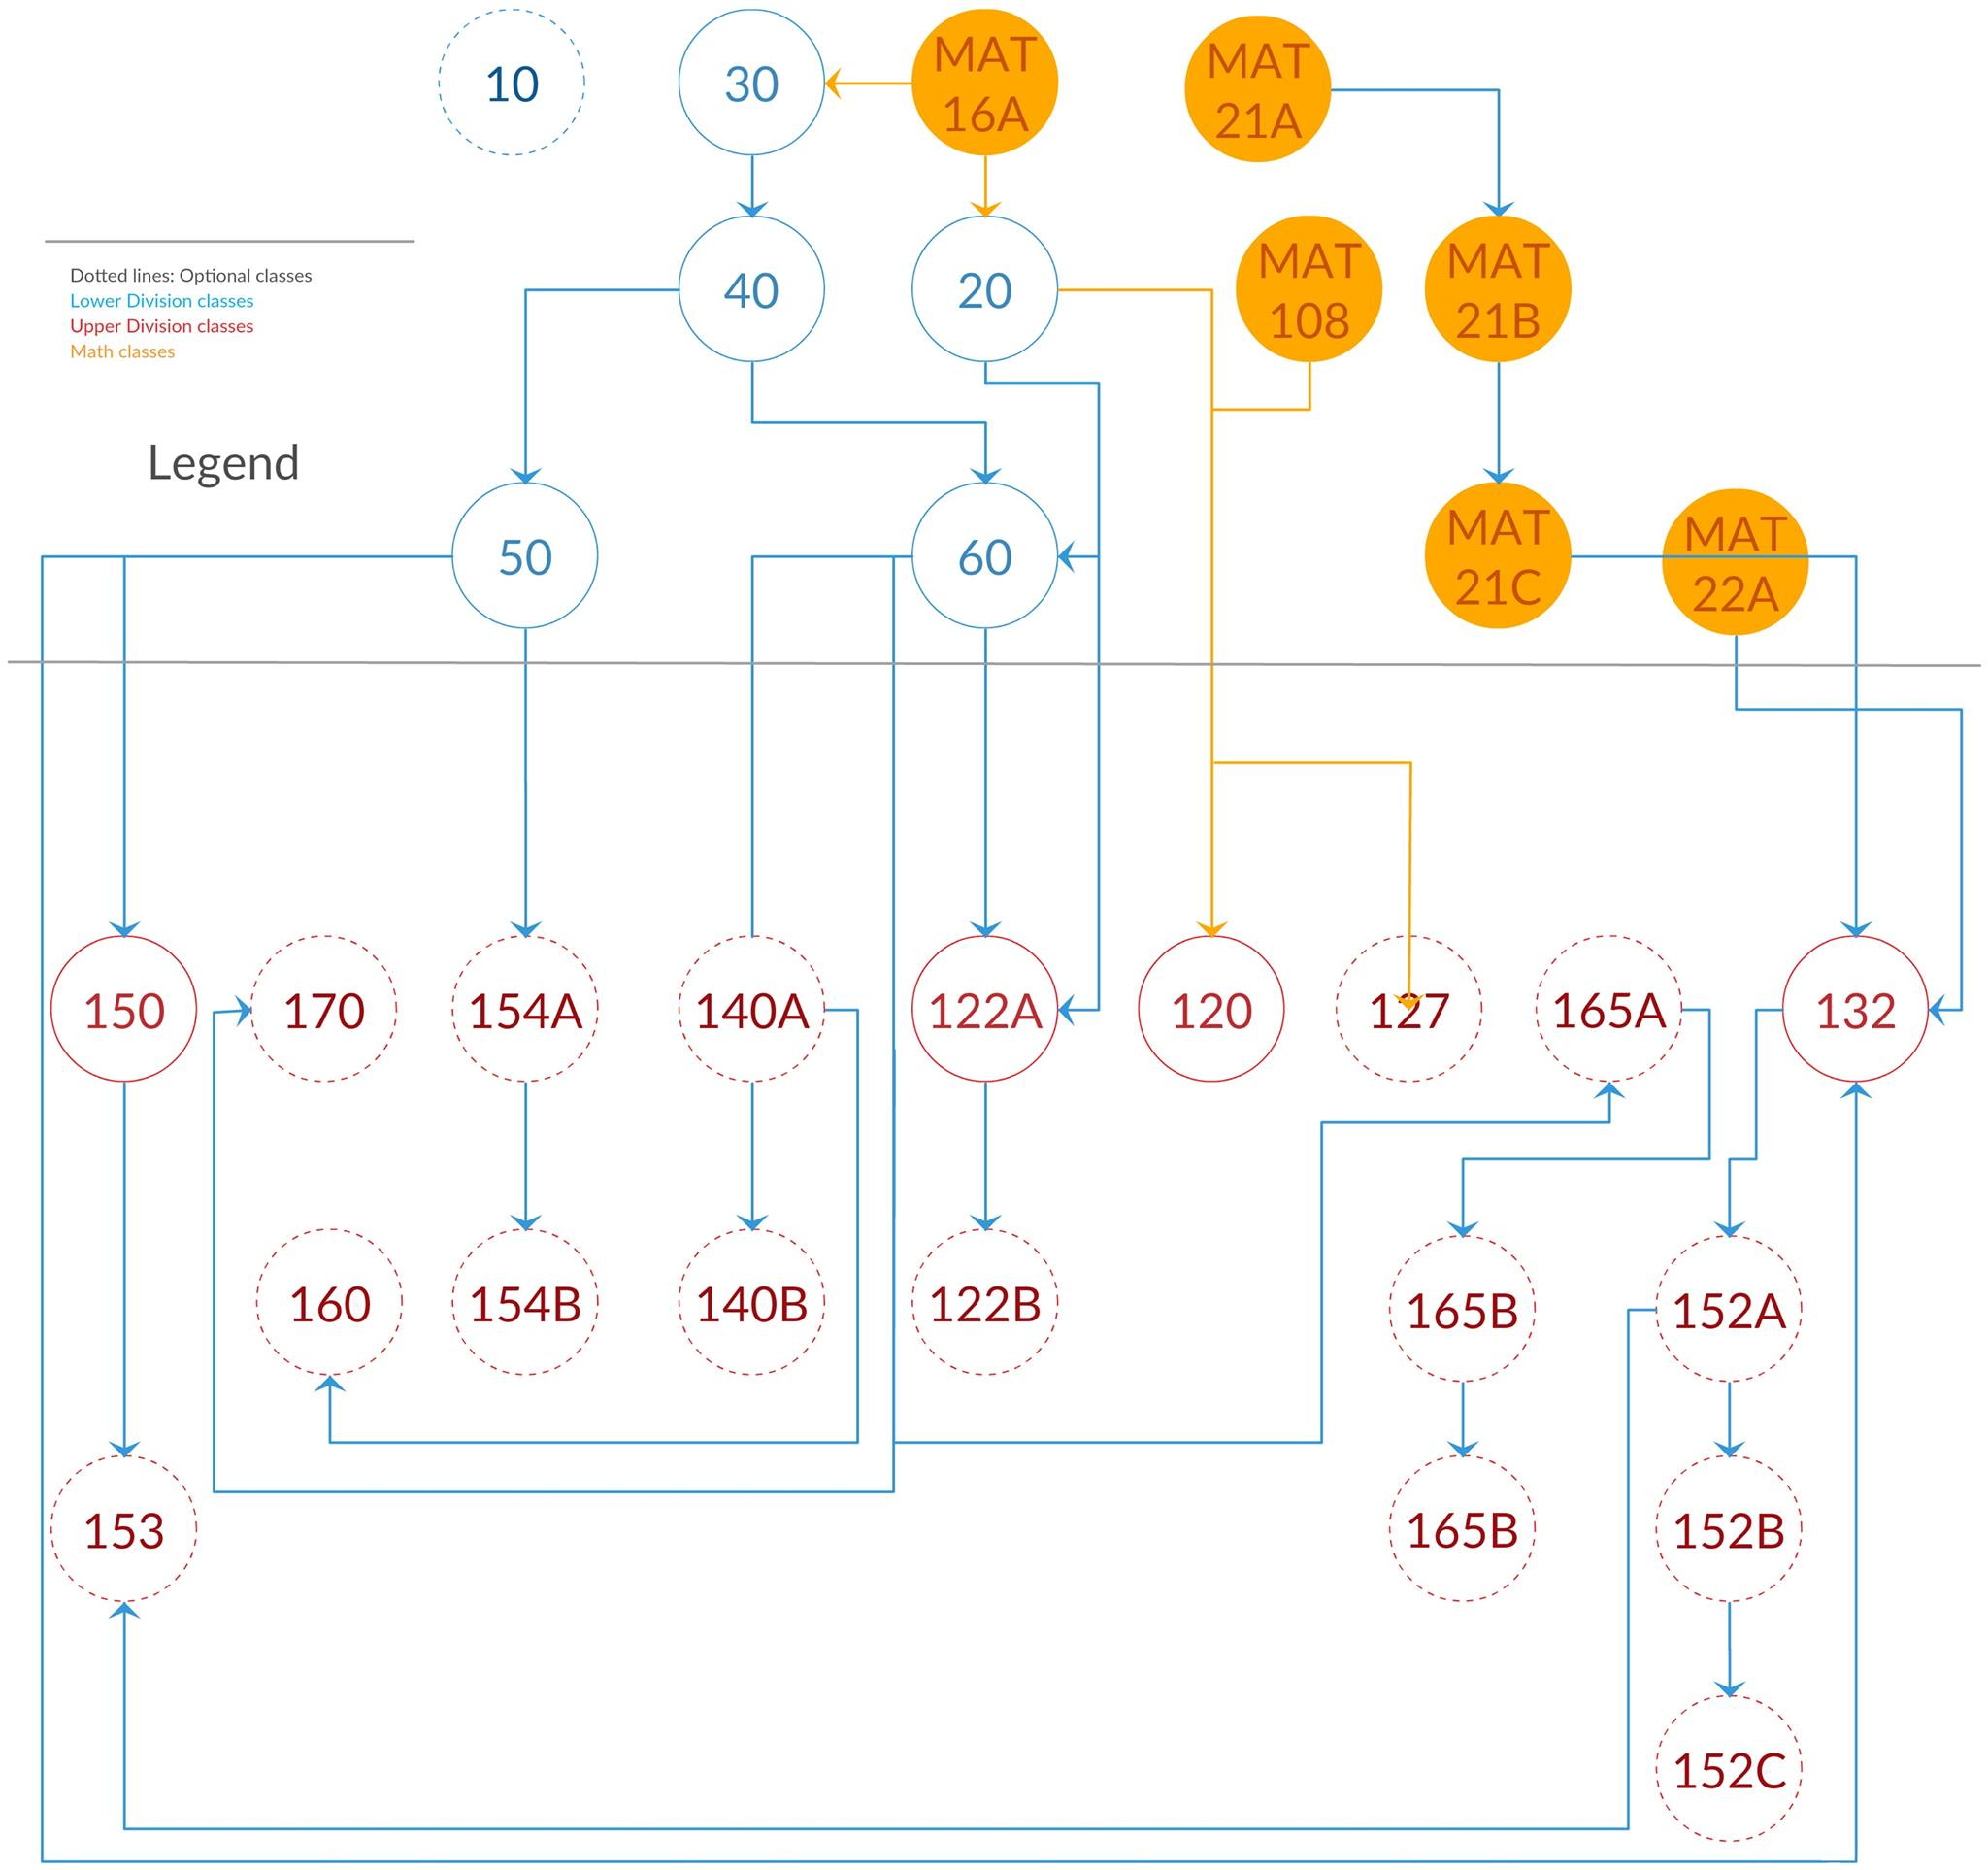
\includegraphics[width=\linewidth]{classdep.jpg}
  \caption{Class Dependency Tree made by David Lin, '17.}
\end{figure}
\newpage
\subsection {FAQ}
\begin{enumerate}
    \item \textbf{What are my chances for getting into x class if I'm position y on the waitlist?}
    \begin{itemize}
        There's no definitive answer for this question. Since CS and CSE are now considered impacted majors, it's probably going to be difficult to get into clasess, especially if you're not a declared CS/CSE major. \\\\ There are some known classes that are more difficult to get into even if you're high on the waitlist, such as core upper division classes and especially ECS 188. If you're a CS major and in need for upper division electives, math upper divs (besides 111) are now an option to replace an upper div elective since catalog 2014. \\\\ Most lower div classes, such as ECS 30, ECS40, and ECS 60, are easy to get into regardless of your position on the waitlist given its high drop percentage and turnover, but there's still no total guarantee. Make sure you have backup CRNs stored up and research other alternative before your pass time! 
    \end{itemize}
    \item \textbf{Can I follow a graduation requirement catalog that's not my own?}
    \begin{itemize}
        You can only graduate from catalogs that have been changed since you started UC Davis -- for example, if Jill started UC Davis in 2013, Jill can follow any catalog changes to graduate after she came in, such as 2014, 2015, 2016, etc. However, Jill is not able to follow any catalog changes from before she came in -- so 2012, 2011, etc are out. 
    \end{itemize}
    \item \textbf {Is my w x y z class load manageable?}
    \begin{itemize}
        That's hard to say. Common classes to take together have been ECS 40 and ECS 20, along with ECS 50 and ECS 60. Depending on professors, some class loads may be more manageable than others.
    \end{itemize}
    \item \textbf{Where can I find tutors for ECS? classes}
        \begin{itemize}
            Please check out \href{https://daviscsclub.org/tutoring/athena}{athena}, our tutor office hours page.
        \end{itemize}
    \item \textbf{How do I get credit for my ECS internship/tutoring/research?}
    \begin{itemize}
        If you're doing research or an internship with a professor or company, click \href{http://www.cs.ucdavis.edu/undergraduate/192-199/}{here} for more information to possibly get credit. If you'd like to tutor with the Davis Computer Science Club and get credits, please either contact the current Tutoring Club Chair at \nameref{sec:officers} or click  \href{https://daviscsclub.org/committee/tutoring}{here}.  
    \end{itemize}
    \item \textbf{How can I prepare for x class?}
    \begin{itemize}
        The best way to prepare for a class is look up the class and find the syllabus. If it's an intro class, try looking up the projects that were done and code up the solutions on your own. ECS 10 uses Python, ECS30 uses C, and C++ is used throughout most of the classes after, such as ECS 40 and ECS 60, and other upper division classes. \\\\
        If you're just starting to take ECS classes, a good way to start is to familiarize yourself with the language and learn the basics: if/else statements, loops, arrays, pointers, and possibly structs or classes. KhanAcademy, Coursera, CodeAcademy, and StackOverflow are good resources for beginners and professionals alike. \\\\
        The various data structures taught in ECS 60 are usually: linked lists (single and doubly linked), stacks, quadratic probing and linear probing hash tables, queues, arrays, and the like.  
    \end{itemize}
    \item \textbf {What are some easy GE's?}
    \begin{itemize}
        Popular GE classes mentioned have been NUT 10, ASA 1/2/3/4, ENL 5F/5P, CLA30, ECM1, COM1/3, ECN1, etc. Alternatively, localWiki has a list of classes 
        \href{https://localwiki.org/davis/Best_Classes_To_Take_Your_Last_Quarter...or_so_I've_heard}{here}.
    \end{itemize}
    \item \textbf {What are some easy or popular math/stat classes to take for that one upper division math elective?}
    \begin{itemize}
        MAT 145 (Combinatorics) and MAT 108 (Discrete Math) are popular options. 
    \end{itemize}
    \item \textbf{What's a good GPA to have for a CS/CSE major?}
    \begin{itemize}
        There's no good answer for this question -- it all depends on what you plan on doing after school. \\\\
        If you plan on going into industry, certain companies may care more about your GPA than others and you may be guaranteed interviews if your GPA is high enough and above a certain cutoff. However, most companies stress personal projects and experience, whether from hackathons, work, or in your own free time, and your GPA isn't much of a deciding factor, if at all. It doesn't hurt to have a high GPA, but in general, it matters more to have projects and experience. From the unconfirmed grapevine, it's been said that anything above a 3.0 is considered decent or competitive, and the few, rare companies that have a GPA cutoff require a 3.0 or above.\\\\
        Graduate school has different requirements and standards and may stress GPA more heavily than industry, but that depends on who you are, which school, and the research you've done. \\\\
        The average GPA for a CS major seems to be around a 2.9, so take with that what you will.
    \end{itemize}
    \item \textbf{What's the best OS/computer/device/etc to own to code with?}
    \begin{itemize}
        There's no 'best' computer or OS to program on or in -- it's all based on personal preference However, if you'd like to try out Linux, the CSIF computers use Linux Fedora (as of now) so that's a good place to start. You can also optionally dual boot or use a Virtual Machine to boot any OS you'd like to test as long as you can get the iso/image for it. \\\\ Popular ones are Linux Ubuntu and OSX. 
    \end{itemize}
\end{enumerate}
\newpage
\section {Hackathons}
\label{sec:hackathons}
\hspace{0.5cm}Hackathon is a conjunction of two words: hack and marathon. Participants can either go solo or form teams and create projects for a certain amount of time, anywhere from 12 to 72 hours. At the end of the hackathon, there's usually a demo session where projects are judged and the best projects take home great prizes. \\

Hackthons are usually hosted by universities or organizations with various company sponsors. Most hackathons are free and provide wi-fi, sleeping areas, food, mentors if you get stuck, and plenty of swag* for everyone to take home. Sometimes hacakthons will provide a certain amount of travel reimbursement for the participant to attend the hackathon.  \\ 

Hackathons are a good way to buff up your resume with projects and expose yourself to more technologies, APIS, and companies. It's also a way to network with other professionals, students, and recruiters in the field. Some companies will recruit and even interview at a hackathon, so if you're looking for job opportunities, keep your resume updated and bring a few hardcopies! \\ 

Contrary to popular belief, anyone can attend a hackathon, even if you're not a computer science major or student. A successful team may need designers, product management leads, and business majors to keep the project going and even if you don't plan to hack on/make anything at the hackathon, attending one and immersing yourself in tech culture is a great learning experience for anyone, so don't count yourself out!

\subsection{A Few Major hackathons}
\begin{center}
    \begin{tabular}{| l | l | l | l |}
    \hline
    Name & Location & theme/requirements & Website \\
    \hline
     HackDavis  & UC Davis     & social good & hackdavis.io \\ 
     SDHacks    & UC San Diego & N/A & sdhacks.io \\
     CalHacks   & UC Berkeley & N/A & calhacks.io/ \\
     SBHacks & UC Santa Barbara & N/A & sbhacks.com/ \\
     HackMIT    & MIT          & N/A & hackmit.org/ \\
     HackDuke & Duke University & social good & hackduke.org/ \\
     TreeHacks & Stanford University & N/A & treehacks.com/ \\
     Spectra    & NorCal       & women only  & sospectra.com \\
     LosAltoHacks & Los Altos & high school students & losaltoshacks.com/ \\
     GunnHacks & Palo Alto & high school students & gunnhacks.com/\\
     HackingEDU & San Mateo    & education & hackingedu.co/ \\ 
     HackTheNorth & University of Waterloo & N/A & hackthenorth.com/ \\
     Stupid Sh*t & San Francisco & useless hacks & stupidhackathon.github.io/ \\
     HackTheLeft & San Francisco & leftist hacks & noisebridge.net/wiki/HackTheLeft \\
     Slash HAck & San Francisco & N/A & hackerearth.com/slash-hack/ \\
     Hackday    & LinkedIn     & bay area interns only &  N/A\\
     \hline
    \end{tabular}
\end{center}
\subsection{Other}
Other places to discover hackathons in your area are: \\ \\
\href{https://mlh.io/}{Major League Hacking} \\
\href{http://eventbrite.com}{EventBrite}

\subsection{Tips}
\begin{itemize}
    \item \textbf{Sleep.} A lot of hackathons stress not sleeping, but four cans of Redbull and working for 9 hours straight can really put a toll on your health and productivity. Find a place to sleep, set breakpoints throughout the hackathon, and just take a shut eye. You'll thank yourself later.
    \item \textbf{Hardcode.} No one comes out of a hackathon with a perfect project. Most of the prototyping comes from hardcoding a bunch of the logic -- a successful hack doesn't come from a perfect implementation, but a good pitch, idea, and appearance. No one, not even the judges, is expecting a perfect product.
    \item \textbf{Winning isn't everything.} You don't have to win a prize in order to call a hackathon succesful for you. If you made something or even learned something, it was a successful hackathon.
    \item \textbf{Network.} Communicate with your team, and other teams, and help each other out! The best part of the hackathon is checking out the demos and seeing what other people have made and talking to other developers about their interests and hacks. It's the best way to learn and expose yourself to other areas in tech.
    \item \textbf{Attend workshops and make use of the mentors.} Most, if not all, hackathons will have a few workshops and mentors. Make use of them -- they're here to help you get through your bugs and guide you through your learning process.
    \item \textbf{Hackathons Demystified.} \nameref{sec:glossary} has a list of terms that you can look over to get familiar with jargon, and has a few other tips to get you prepped! 
\end{itemize}

\subsection{FAQ}
\begin{enumerate}
\item \textbf{I'm not 18+, can I still attend a hackathon?}
    \begin{itemize}
    Yes, you can! There are plenty of hackathons that allow attendees other 18. There are high school hackathons and hackathons that allow minors, such as /hack. Keep a lookout for them!
    \end{itemize}
\item \textbf{How much does it cost to attend a hackathon?}
    \begin{itemize}
        Hackathons are usually free, unless otherwise specified. Professional hackathons can cost money, so contact the hackthon's organizers for more details. 
    \end{itemize}
\item \textbf{What should I bring to a hackathon?}
    \begin{itemize}
       Your laptop, charger, ID, a creative spirit, and anything else you need to hack with! If it's an overnight hack, blankets, sleeping bag, toothbrush/toothpaste and any hygienic products would also be recommended.
    \end{itemize}
\item \textbf{I've never coded before/I'm a beginner/I'm scared to drag my team down -- can I still go to a hackathon?}
    \begin{itemize}
        Yes, yes, yes! Hackathons are for everyone regardless of experience. In fact, beginners are highly encouraged to attend. If you\'re worried about not knowing anything, find likeminded beginners and form a team with them. Hackathons are all about learning, so don't be afraid if you don't know anything!
    \end{itemize}
\end{enumerate}

**swag: free goods (branded or otherwise) from companies or universities, like tote bags, blankets, water bottles, t-shirts, stickers, toothbrushes, etc. 
\newpage

\section {Applying For Jobs and Internships}
\subsection{How and Where to Apply}
\hspace{0.5cm}There's a few way to apply and score \nameref{sec:interviews}. 
\begin{enumerate}
    \item Cold Applying
    \item \nameref{sec:referrals}
    \item \nameref{sec:careerfair}
\end{enumerate}

Cold applying is going to each company's website or portal and applying. The top ones to hit up every year are always the major companies: Google, Facebook, Amazon, Apple, and Microsoft. Always apply, even if you don't think you have a chance -- they'll keep your resume and profile in their archive for a while and, in the future, they might look you up and reach out to you! If you think of a company you might want to work for, look them up and apply to them!\\

\textbf{Tip}: Keep a spreadsheet of the ones you've applied to, the positions you've applied to, the date you applied, and the status of your application. If it's been a few days since you've heard from your recruiter, make sure to follow up! \\

Before you apply, however, you're probably going to need at least a resume, and maybe a cover letter.
\subsection{Resume}
\label{sec:resume}
\hspace{0.5cm} The sections of a tech resume can be broken down like so: 
\begin{enumerate}
    \item Name and Contact Information (email, phone, Github, LinkedIn, website)
    \item Skills (languages, libraries, frameworks)
    \item Projects (school, hackathons, personal) 
    \item Experience (mostly tech, if possible, and/or leadership/volunteering)
    \item Education (major(s) and minor(s), graduation year, GPA optional)
    \item Relevant Coursework (optional)
\end{enumerate}

You should definitely include your Education and GPA, the latter being optional and only if your GPA is decent, but neither are particularly interesting unless either are truly exceptional, so put your skills, projects, and experience at the top as much as you can. \\

Relevant Coursework is also good section to also add, especially if you're looking for an internship or full-time position and don't have much experience under your belt. Any CS classes you've taken or are projected to take in the next quarter, especially Data Structures and Algorithms, are always good classes to add.  
\subsubsection {Building Your Resume}
\hspace{0.5cm} If you haven't taken many classes or have skills or relevant experience (which most people don't when they try and find internships or jobs, so don't worry), you're going to have to start by building projects. \\

You can build projects by going to \nameref{sec:hackathons}, making your own website or app, contributing to open source projects, etc. It doesn't have to be big. You can make a Unitrans app, a Tic Tac Toe app, a Google Chrome extension, your own website, or anything simple (or complicated) to learn and show initiative and incentive. See below at \nameref{sec:projects} for more ideas. \\\

You can also build your resume by taking more classes. Your UC Davis classes aren't the only ones you can add to your resume -- in your free time, taking an online Coursera class or two and finishing the course is also something you can add to your resume. Keep in mind that some Coursera classes are free, and some are not. \\

Please also check \nameref{sec:onlinepresence} to build your resume and online presence. \\

Even if you don't have many projects, classes, experience, or skills, it doesn't mean you shouldn't still try your luck at applying! It's always good to gain experience in applying for jobs and networking.  
\subsubsection{Resume Tips}
\begin{itemize}
    \item If you have a lot of experience, choose a few and tailor your resume for the job you're applying for.
    \item The general rule of thumb is one page for every ten years of relevant experience and if you're applying for a new grad or internship position, keep it to one page. If a recruiter can't skim your resume and read everything quickly, then it's most likely going to be tossed or archived.
    \item Black type on white paper. Size 10 font, minimum. Half inch margins, minimum. Equal borders and spacing for all items. Your wording should be concise, legible, but have brevity. Your resume can be pretty, but it doesn't have to be a work of art. Keep it straightforward and neat -- all your information should be easily found.
    \item Stretch your content across the page -- white space should only be used to separate your content for legibility -- you don't need splotches of white space on your page for no reason. It makes it look like you don't have enough. \\\\ You can always fill up your resume with something, whether skills or projects or coursework or experience. If you don't have any of those, learn them, build them, take them, get them. 
    \item Other items you can include in your resume: awards, honors, scholarships, fellowships, publications, research, interests, etc.  
    \item You don't need to put communication, leadership skills, or anything similar as your skills -- that's either evident through any large scale team projects you've listed or it'll be evident enough enough during a phone and onsite interviews. \\\\ There's also no need to put Microsoft Word, Powerpoint or anything similar as your skills unless the position specifically asks: most people know Microsoft Word and if not, they can quickly learn. \\\\
    There's also no need to put Objective as a section either -- it's outdated. References is also not a needed section if you're going to write 'Available upon request' -- recruiters will ask for a reference or a background check if they need one from you. 
    \item Microsoft Word with tables is the most commonly used software to make resumes, and some people also choose to use LaTeX
    \item Formats can change with every file extension and version, so try to keep an edited version (in Word or LaTeX) and send recruiters the PDF version of your resume. 
    \item Don't put your address. No one contacts anyone for job opportunities via address anymore and if recruiters need your address, they'll ask. Leaking your address is a dangerous potential for identity theft -- your phone number, email, and any social networking sites (LinkedIn, Github, your website, etc) should suffice as contact information.
    \item Keep descriptions of each position you've held short -- two to three bullet points at most, with a line each. A good description should be like what Churchill said about speeches and skirts: "long enough to cover everything, but short enough to be interesting". 
    \item If possible and space permits, it's also nice to include one position you've held that is not tech related -- it shows that you have interests outside of tech. For example, if you volunteer at a children's center for reading, or held a leadership position in a running club.  
    \item Check for typos! Don't lie! These are the big ones that can be easily fixed!
    \item Keep your name large, nice, and bold -- it makes you memorable.
\end{itemize} 
\subsection{Cover Letter}
\hspace{0.5cm} A general template for a cover letter looks something like this:
\begin{enumerate}
    \item Dear XYZ,
    \item Your name, introduction, the position you're applying for, how you heard about the company (especially if it's through referral), and anything you know about the company.
    \item A short discussion about your relevant skills, projects, and skills and what you can bring to the company technical skills wise. What challenges you think the company faces and what interests you about them, and how passionate you are about their product. Do some research here.
    \item An optional paragraph on your leadership skills, collaborative skills, various interests, and what you can bring as a leader or team member to the company.
    \item Ending note, conclusion, and state that you believe your attached resume (or website, or whatever you choose) will highlight any of your other qualities. Thank them for their time.
    \item Sincerely, Your Name
\end{enumerate}

You shouldn't have to write a brand new cover letter for every company you apply to. Your cover letter should be a malleable template and only changed a little for every company -- keep the main details the same, such as your skills, but do some research and add or change details about the company you're applying to as you see fit.\\

Your cover letter should also be one page, and should contain the same header as your \nameref{sec:resume} (Name and Contact Information).

\subsubsection{Cover Letter Tips}
\begin{itemize}
    \item If they ask for an optional cover letter, include your cover letter. You're going the extra mile to show them you want the job -- do it. 
    \item Check for typos! Don't lie! Be consistent with your resume! 
    \item Don't rote list your resume out -- your cover letter is supposed to add to your resume, not be a summary. Add details that can't be seen on your resume, such as what you enjoyed most about a project or class or what kind of technology stack you've worked with and are learning.
\end{itemize}
\subsection {Referrals}
\label{sec:referrals}
\hspace{0.5cm} This is the best way to get an interview. Your application is sent to the top of the stack and recruiters will review referred applicants first opposed to those that cold apply. It's sad, but true. Network, network, network -- make friends in your classes, make friends at hackathons, make friends at work. These people will get jobs and these are the people who can push your career forward someday.\\

It's also, well, just nice to have friends in tech. :) And don't forget to return the favor and refer them when you get a job as well!  
\subsection{Career Fairs}
\label{sec:careerfair}
\hspace{0.5cm} UC Davis has several career fairs in a year, and one specialized just for engineering, with a list of them here: \href{https://icc.ucdavis.edu/employer/fairs.htm}{Career Fairs}.\\

If you're actively looking for a job or internship, go to career fairs! Dress business formal/casual, print 15-20 resumes, research the companies you want to talk to, get there early if you can, and start hitting up each recruiter and talking to them. Even if you're not looking for a job at the moment, you can just go and pick up all the swag* the companies are handing out.\\

One thing to do before a career fair is to practice your elevator pitch. It's a 1-2 minute spiel about yourself that goes something like this:\\

\textit{Hi, my name is Jill, I'm a 2nd year and I study Computer Science and Engineering at UC Davis. I'm really interested in your Test Automation Internship position. I've known about X company for a long time and I'm very passionate about your product. Can you tell me more about yourself and the various positions and X company?}
\subsection {Online Presence}
\label{sec:onlinepresence}
\hspace{0.5cm} The first thing a recruiter does is look at your resume. Then they either see if you have any more information (website, LinkedIn, Github, Devpost, etc) on your resume that they can check online for and if not, they Google you. You're going to seem less appealing than a candidate who has a fleshed out online presence that the recruiter can get to know, so building your presence as soon as you start applying for jobs is key. \\

You should make a: 
\begin{enumerate}
    \item LinkedIn
    \item Github
\end{enumerate}

and optionally, a website or portfolio. \\

Your LinkedIn should not only reflect your resume, but anything else you didn't have a chance to add on your resume, such as classes, more details on any projects you've done, other work or volunteering experience, etc. It should be detailed and thorough, with any images or links to projects you have, along with any coursework you have. Recruiters will often look at your LinkedIn and may contact you from there. \\

Your Github should have all your personal projects and code samples. If you don't know what to add, try solving some interview problems on sites such as HackerRank or Project Euler and putting it in a repository. \\ 

Your website, if you decide to make one, doesn't have to be fancy -- it can be merely a static page with your name, your email, your LinkedIn and Github and any relevant websites. You can talk about your interests, volunteering, work history, hackathons you've attended, projects you've made, etc. It's your website, but also your portfolio and a chance to show off your technical skills. See more at \nameref{sec:website}. \\

Other ways you can build your online presence is being active in various other communities, such as StackOverflow or StackExchange, or contributing to various open source communities.\\

\textbf{Note:} The Davis Computer Science Club does not advise putting projects done from classes on Github -- it is, unfortunately, common for students to cheat and plagiarise from code past students have made available online.
\subsection {Website/Personal Portfolio}
\label{sec:website}
\hspace{0.5cm} If you've never built a website before, here's the place for you! The easiest place to host your website is at: \href{https://pages.github.com/}{Github Pages} and they have a convenient and simple tutorial. \\

A few suggestions to drum up your website are to use \href{http://getbootstrap.com/2.3.2/}{Twitter Bootstrap} for the styling. Bootstrap is merely a set of CSS stylesheets you can use from, and you can download it from the link given or use any of the CDNs provided (more on the link).
\subsection {Negotiating Offers}
\hspace{0.5cm} You should always try and negotiate your base pay, stock options, or benefits. In fact, most companies expect you to. \\

If you have another offer that's paying you more, you should definitely ask if the offer you're looking at if they can possibly match or exceed the offer of the other company.\\

You'll get more leverage if you have another offer, but by itself, you can leverage your skills and ask for more. Just simply ask your recruiter (nicely!) if they can possibly raise your base salary/benefits/etc since it seems a bit low. Most people seem afraid they're going to seem like an ungrateful money-grubber -- you're not. It doesn't matter if you like the company or the product, there's nothing wrong with having more money and there's no harm in asking: you already got the offer! \\

If there's a certain salary/benefit/stocks combination you should definitely not go below, a number that you should determine by yourself based on research, try and keep to it. If you know the recruiter is offering you too low of a sum and they refuse to raise your offer, decline and interview elsewhere. Don't shortchange your worth just for the experience. You'll get other offers.
\subsection {Rejection}
\hspace{0.5cm} It happens to everyone. They say that the first rejection is the hardest, but I find that all the subsequent rejections hurt as much, if not more. But it literally happens to everyone -- the best engineers get rejected, and often. No one gets to where they are without it. \\

Some companies won't send a rejection letter. Some will. Both of them suck. Sometimes you won't even know why they don't want to hire you, and they could be for completely arbitrary, stupid reasons, like the recruiter just had a bad day or they misplaced your paperwork. It could be that another candidate was just too good -- maybe they were a student from MIT with 22 papers under their belt and they've been coding since they could walk how could you possibly compete with that? And yes, they can be for technical reasons: your solution wasn't optimized enough, you couldn't find the edge cases, your skills aren't developed enough. Most companies won't tell you.\\

Take it as a learning experience to grow more. It's okay to cry. It's okay to feel like crap for a few days. But in the end, it's just another experience. It doesn't mean you're not going to get a job or that you can't apply again. It's not personal. You're smart, you're funny, you're likeable, and you're going to make it in the end.
\subsection {Resources} 
\href{https://github.com/j-delaney/easy-application}{List of Easy Applications}
\subsection{Tips}
\begin{itemize}
    \item Recruiters are people, too. Be nice to them. Thank them, and often. Thank your interviewers, too. Err on the side of being too polite, always.
    \item Follow up with your recruiter -- if they haven't responded in a few days to a week about your interview or the next steps, email them again. And again. Call them, email other people from the company, and leave messages if you have to. 
    \item A few good questions to ask your interviewer (pick and choose), technical or otherwise, at the end of the interview are:
    \begin{itemize}
        \item What do you like about X company? 
        \item How is X company different from other companies?
        \item What team do you work on at X company? What do you do?  
        \item What's the culture like at X company?
        \item What's the technology stack at X company/your team like?
        \item How flexible is X company with changing teams or learning new things? 
        \item What are some skills or values every intern/employee should have at X company?
        \item What are the next steps of the process?
    \end{itemize}
    \item Attend conferences or hackathons not just for the learning experience, but to network! 
    \item \href{http://engineering.ucdavis.edu/corporate-relations/student-recruitment/company-tours/}{UC Davis College of Engineering} offers a few industry tours a year (such as Square, Google, Apple, etc), so if you're interested in taking a look inside at some pretty great companies, follow their Listserv or contact COE! This is open to UC Davis students based on a first come first serve basis. 
\end{itemize}
\subsection{FAQ}
\begin{enumerate}
    \item \textbf{Should I put code I've written for class projects on my Github?}
    \begin{itemize}
        That's up to you. DCSC does not advise or endorse this, however -- while it's a quick way to show your code snippets and many students do so, but at full disclosure, other students may look up your code and copy, so you might be at risk with the SJA. Posting your professor's code that you built upon and calling it your own may be considered plagiarism, so if you are going to do so, you might want to put a disclaimer. 
    \end{itemize}
    \item \textbf{When should I start applying for jobs and internships?}
    \begin{itemize}
        There's no 'should' or supposed timeline -- just whenever you're comfortable! However, you can apply for internships starting your freshman year if you'd like. It's recommended to only start applying after you've taken ECS 60 Data Structures or already have a foundation in Data Structures, as most of your interview questions will be based on that. 
    \end{itemize}
\end{enumerate}
**swag: free goods (branded or otherwise) from companies or universities, like tote bags, blankets, water bottles, t-shirts, stickers, toothbrushes, etc.
\newpage
\section {Interviews}
\label{sec:interviews}
\hspace{0.5cm}Most interviews for software engineering or related positions are split between two kinds of questions: behavioral and technical.  

\subsection {Interview Formats}
\begin{itemize}
    \item \textbf{Coding Challenge}
    \begin{itemize}
        \item You'll be given the challenge in the form of a link, such as HackerRank, where you have to complete a certain number of problems in a given amount of time (30 minutes to a few hours, usually) by a certain deadline. \\\\ Make sure your laptop or computer is charged and you find an ideal and quiet place with internet to work and turn off any distractions for the amount of time you're interviewing. Once you start, you can't pause, so make sure you're ready.
    \end{itemize}
    \item \textbf{Remote/Phone Interview}
    \begin{itemize}
        \item This can either be a behavioral or technical interview and it's usually done via phone or video chat. There might be multiple rounds, sometimes back to back or spread out through several weeks or months. Always be prepared for both types of questions as you never know what they're going to throw at you. \\\\
        If it's a technical phone interview, interviewers may ask you questions straight up, or ask you to code up a more complicated problem on a shared document such as GoogleDocs or CodePad. You may have to run the code after you're done, so code carefully if you don't want to spend most of your interview debugging.
    \end{itemize}
    \item \textbf{Onsite} 
    \begin{itemize}
        \item If you were invited to an onsite, you're probably close to the end! Be prepared to spend a few hours/the whole day at the onsite location, and get there early if you can. An onsite usually has whiteboard coding and debugging the code with the interviewer in the room.\\\\
        Depending on the company, you might interview with other candidates, have back to back rounds, have multiple onsites, or just have one interview. Either way, be prepared for the worst and practice, practice, practice. \\
    \end{itemize}
\end{itemize}
\subsection{Common Interview Questions}
\begin{itemize}
    \item \href{http://www.forbes.com/sites/jacquelynsmith/2013/01/11/how-to-ace-the-50-most-common-interview-questions/#f57f0c348737}{Behavioral} 
    \item \href{https://www.reddit.com/r/cscareerquestions/comments/20ahfq/heres_a_pretty_big_list_of_programming_interview/}{Technical}
\end{itemize}
\subsection{Resources and Practice}
\begin{tabular}{|c|c|p{6cm}|}
\hline
    \textbf{Title} & \textbf{URL} & \textbf{Description}  \\
    \hline
    HackerRank & http://hackerrank.com & various interview questions from trees to data structures to databse questions in any language you choose \\
    \hline
    GeeksForGeeks &http://www.geeksforgeeks.org/ & lots of interview questions and their solutions in different languages\\
    \hline
    ProjectEuler & https://projecteuler.net/ & programming and math challenge questions. Google's advised website to check out for programming questions. \\
    \hline
    LeetCode & https://leetcode.com/ & various problems and their solutions (with some digging) \\
    \hline
    CareerCup & https://www.careercup.com/ & programming problems and solutions in a stackoverflow like format\\
    \hline
    Reddit Programming Questions & reddit.com/r/dailyprogrammer/ & problems on reddit and people answering solutions, ranked easy - hard\\
    \hline
    Glassdoor & http://glassdoor.com & look up the company you're interviewing for and various questions they may have \\
    \hline
    Cracking the Coding Interview & N/A & a book with programming questions, hints, and solutions  \\
    \hline
\end{tabular} \\ \\ \\
\href{http://bigocheatsheet.com/}{Big-Oh}\\
\href{https://gist.github.com/TSiege/cbb0507082bb18ff7e4b}{Interview Cheat Sheets}

\subsection {Tips}
\begin{itemize}
    \item \textbf{Think out loud.} If you're given a problem, think out loud and explain your thought process before starting. Don't be afraid to ask your interviewer questions if you're stuck or don't understand the problem -- they don't want to see just your speed/efficiency in coding, but whether you're able to collaborate with other people to figure out the problem. 
    \item \textbf{Optimize.} You're probably going to be asked what are the edge cases and Big-Oh of your solution and whether you're able to optimize your code further. When you're practicing for interviews, make sure you ask yourself these questions and try and optimize your code as much as you can. When in doubt, see if you can use a hash map or hash table. 
    \item \textbf {Bruteforce, then optimize.} If you're truly stuck on a problem and how to get it to a nice optimization in regards of speed and memory, think of the worst solution you can then start from there and ask yourself: what's the bottleneck (slowest part/congestion) of this solution? How can I optimize this further? 
    \item \textbf{Sleep.} This goes without saying, but get plenty of sleep before your interview. It's hard to code when you're nervous already; there's no need to add sleep deprivation to the mix.
    \item \textbf{Practice with friends.} Or go to Mock Interview sessions! Simulate an interview environment as much as you can and take turns asking each other questions, both behavioral and technical. It'll help you get into the rhythm and the types of questions asked.
    \item \textbf{Choose a language you're comfortable with.} If you're not sure which to choose, the most common language I've seen people interview with have been Python and Javascript. They're both clean scripting languages with simple and easy-to-remember syntax and implementing data structures is pretty cake with both. However, you may not always get a choice in what language you can interview in and some interview questions may be better written in other languages. Play to your strengths.
    \item \textbf{Don't neglect the behavioral!} A lot of companies stress culture fit and people want to hire who they want to work with. Learn how to pitch yourself and practice not just your marketing your skills and projects, but who you are as a person. Don't be afraid to talk someone's ear off about your hobbies and anecdotes -- chat with your interviewers. They're people too.
    \item \textbf{Don't stop practicing.} If you plan on entering the tech industry in the future and continuing with it, you're going to be interviewing quite often. Always refresh yourself on your data structures and problem solving skills, and keep with it.
\end{itemize}
\subsection{FAQ}
\begin{enumerate}
    \item \textbf{There's so much material to cover, where should I even begin?}
    \begin{itemize}
       Start with reviewing any material you have from ECS 60 (Data Structures). Most websites or books about interviewing begin with easier questions so progress from there -- when you've gotten the hang of solving simple questions, try out a few moderate-hard questions, think of your own solution and optimization, test your solution, then look at other people's answers.\\\\Some times the best way to learn is to look at some of the ways other people use to solve their problems. After looking at their solution, code it up in a different language and test it. Then another. Keep going. Rinse and repeat. 
    \end{itemize}
    \item \textbf{What should I know for an interview?}
    \begin{itemize}
       General knowledge everyone should know: data structures -- arrays, hashes, heaps, lists, queues, stacks, trees; strings; graphs; bit manipulation, Huffman encoding, and the like. It also depends on what position you're interviewing for. \\\\For example, an interview for a front-end position may ask you primarily HTML/CSS questions. In fact, any skill you put on your resume as something you know or proficient in is fair game. 
    \end{itemize}
    \item \textbf {How should I dress/look for an interview?}
    \begin{itemize}
        Business formal at best, business casual at worst, unless otherwise specified. If it's a video interview, dress up as well, at least from the waist up. 
    \end{itemize}
\end{enumerate}
\newpage
\newpage
\section {Techincal Skills}
\hspace{0.5cm}Some technical skills, languages, and frameworks that are out there and trending right now! These are only a subset of technologies that exist, so if you're interested, feel free to do some research on your own. :) 
\subsection{Languages}
 \hspace{0.5cm} Depending on what part of software you'd like to get into, some may be more relevant or useful than others. You do not need to know ALL of these languages to be considered competitive! These are also just a small list of popular languages used today. Please Google them for more information.\\
\begin{center}
\begin{tabular} {|p{3cm} |p{8cm}|}
\hline
\textbf{Language} & \textbf{Description}\\
\hline
C & Low level language. You'll usually touch C if you're writing firmware or directly interacting with hardware.\\ 
\hline
C++ & Improved C with classes, a standard library, and extra features. Used maninly to communicate with hardware.\\ 
\hline
Java & Popular cross-platform programming language. Code once, run using a virtual machine in all major platforms. Has a large overhead due to this fact.\\
\hline
Javascript & The scripting language in your browser. Can be emulated on your desktop. Worth learing if you want to do web development.\\
\hline
Visual J\# & Microsoft's version of Java. Please let it die.\\ 
\hline
HTML/CSS & The staple of web development. HTML is for creating structure, CSS is for applying style to those structures\\
\hline
Python & Quick and easy programming language. Easy to prototype functions, perfect for job interview questions. Become a Python 3 master and you won't regret it!\\
\hline
SQL & Database manipulation language. Used Insert, update, change, and retrieve data inside a database. A staple of backend developers.\\
\hline
Ruby & Like python, but worse. It's a simplistic but powerful language.\\
\hline
PHP & It's basically C, but used for web applications. Excessive use of the dollar sign for variablenames will make you feel filthy rich.\\
\hline
Perl & Command line scripting language. Can be used in conjunction with command line tools to manipulate data or files.\\
\hline
R & If you're into math, stats, or physics, (or your name is Matloff) R is your best friend! It's the perfect language for your graphing or calculation needs.\\
\hline
Swift & Language used to create apps that work on Apple products.\\
\hline
Objective C & An alternative to Swift. Will mess with your mind.\\
\hline
Matlab & Use R.\\
\hline
RegEx & Pattern matching for strings. Can validate a string or extract/manipulate certain subsets of strings.\\
\hline
\end{tabular}
\end{center}
\hspace{0.5cm} If you'd like to know more, other people have written better lists and descriptions  \href{https://www.quora.com/What-are-the-pros-and-cons-and-uses-of-the-major-programming-languages}{here} and \href{https://www.quora.com/What-are-the-pros-and-cons-and-uses-of-the-major-programming-languages}{here}. 
\subsection{Text Editors}
\hspace{0.5cm}There's a lot of argument on what's the best text editor to use, but here are some popular ones. Optionally, you can choose to use an IDE. Here are a few! 
\begin{itemize}
    \item Sublime 
    \item emacs
    \item vim, vi
    \item gedit 
    \item atom editor
\end{itemize}
\subsection{Frameworks}
\begin{tabular}{|c|c|}
\hline
\textbf{Framework} & \textbf{Language} \\
\hline
Javaspring & Java  \\
\hline
Spark & Java  \\
\hline
Ruby on Rails & Ruby  \\
\hline
Sinatra & Ruby \\
\hline
Django & Python  \\
\hline
Flask & Python  \\
\hline
Node.js & Javascript  \\
\hline
React & Javascript  \\
\hline
Angular.js & Javascript  \\
\hline
Bootstrap & HTML/CSS  \\
\hline
Semantic UI & HTML/CSS \\
\hline
\end{tabular}

\subsection{FAQ}
\begin{enumerate}
    \item \textbf{What language should I learn first?}
    \begin{itemize}
        It honestly depends on what you'd like to get into! Most people start off either learning C, C++, or Python, as they're good beginning languages to learn from, but honestly any language is a good start. 
    \end{itemize}
\end{enumerate}
\newpage
\section{Building Projects}
\subsection {Project Ideas and APIs}
\label{sec:projects}
\hspace{0.5cm} Keep in mind these are meant to be simple ideas to get you started with creating a project on your own. Most, if not all of these, can be either developed into a phone application or a web application, or whatever you prefer. Get creative! They can be quirky, fun, or interesting. :) \\

Any ideas from other people are meant for inspiration only -- do not take their code and claim it as your own. That's lying and famously called plagiarism, people. 
\subsubsection{Project ideas or inspiration}
\textbf{ideas}
\begin{itemize}
    \item a tic tac toe application
    \item a unitrains/bus application
    \item a spellcheck application
    \item a Pokemon weakness/strengths application
    \item a basic social networking site
    \item bill splitting for roommates
    \item a calculator
    \item an exam grade calculator 
    \item an app that tells you if you should wear shorts or pants in the morning
    \item a weather app based on location
    \item \href{https://github.com/karan/Projects}{project ideas, with examples}
\end{itemize}
\textbf{inspiration:}
\begin{itemize}
    \item \href{https://jenniferdewalt.com/}{180 websites in 180 days}
    \item \href{http://drakeweather.com/}{checking weather with Drake}
    \item \href{https://github.com/cathydeng/are-men-talking-too-much}{website that tracks the time each gender speaks}
    \item \href{https://github.com/panicsteve/cloud-to-butt}{chrome extention that changes all instances of cloud on the page to butt}
\end{itemize}
\subsubsection{Useful APIs}
\href{https://github.com/toddmotto/public-apis}{Public and Free APIs}
\subsection{FAQ}
\newpage
\section {For Marginalized Folks in Computer Science}
\hspace{0.5cm} A few resources and clubs exist for those not commonly represented in the tech industry. 

\subsection{A Few Clubs On Campus at UC Davis}
\begin{tabular}{|p{5cm}|l|p{7cm}|}
\hline
\textbf{Name} & \textbf{Identities} & \textbf{URL} \\
\hline
Society of Women Engineers (SWE) & women, engineering, CS included & swe.engineering.ucdavis.edu/ \\
\hline
WiSTEM & women, stem & facebook.com/wistemucdavis/ \\
\hline
Pilipinx Advancing Science Engineering (PASE) & pilipinx, STEM & joinpase.weebly.com/ \\
\hline
Black Engineers Association & black, engineering & http://beaucdnsbe.weebly.com/ \\
\hline
The American Indian Science and Engineering Society (AISES) & native american, STEM & http://aises.engineering.ucdavis.edu/ \\
\hline
Chicano and Latino Engineers and Scientists Society (CALESS) & chicanx/latinx, STEM & caless.engineering.ucdavis.edu/ \\
\hline
Queers in Science Club & queers in STEM & N/A, check with LGBTQIARC\\
\hline
BlackOut & black, queer & N/A, check with LGBTQIARC \\
\hline
La Familia de UC Davis & latinx/chicanx, queer & facebook.com/groups/2234329547/ \\
\hline
Asian Pacific Islander Queers & AAPI, queer & facebook.com/groups/APIQatUCD/ \\
\hline
Queer Student Union (QSU) & queer & N/A, check with LGBTQIARC \\
\hline
\end{tabular}

\subsection{Centers and Counseling}
Alternatively, the centers on campus are also helpful for general needs. There are CAN advisers at every center that can aid y'all with counseling and advising. The CCC, LGBTQIARC< and SRRC are located in the Student Community Center at UC Davis. The WRRC is located in North Hall.\\ 

\begin{tabular} {|p{8cm}|c|}
\hline
\textbf{Name} & \textbf{URL} \\
\hline
Cross Cultural Center (CCC) & ccc.ucdavis.edu \\
\hline
Women's Resources and Research Center (WRRC) & wrrc.ucdavis.edu\\
\hline
Lesbian, Gay Bisexual, Transgender, Questioning, Intersex, and Asexual Resources Center (LGBTQIARC) & lgbtqia.ucdavis.edu \\
\hline
Student Resources and Retention Center & srrc.ucdavis.edu \\
\hline
Student Counseling & shcs.ucdavis.edu/counseling-services \\
\hline
\end{tabular}

\subsection {Other Resources} 
A few other resources and organizations on campus can be found at the following links:  \\

\href{https://www.ucdavis.edu/admissions/undergraduate/community/african-american-student-resources/}{UC Davis African American and African Student Resources}\\

\href{https://www.ucdavis.edu/admissions/undergraduate/community/latino-chicano-organizations/}{UC Davis Chicanx/Latinx Student Resources}\\

\href{https://www.ucdavis.edu/admissions/undergraduate/community/}{UC Davis Multicultural Student Resources}\\

\href{http://lgbtqia.ucdavis.edu/connected/student-org.html}{UC Davis Queer Student Resources}\\

\href{https://github.com/cristianoliveira/awesome4girls}{Resources for Women in Tech} \\

\href{http://peopleofcolorintech.com/}{People of Color in Tech}\\

\href{http://ghc.anitaborg.org/}{Grace Hopper: Celebration of Women in Computing Conference}\\

\href{https://github.com/freialobo/GHC-Scholarships}{Grace Hopper Conference Scholarships List}\\
\subsection{FAQ}
\newpage
\section{Glossary}
\label{sec:glossary}
\hspace{0.5cm} Here are some definitions and jargon that you may have heard before, but weren't sure what they were. \\

Attached is a pdf from Carnegie Mellon University's Hackathons Demystified workshop with a glossary. \\
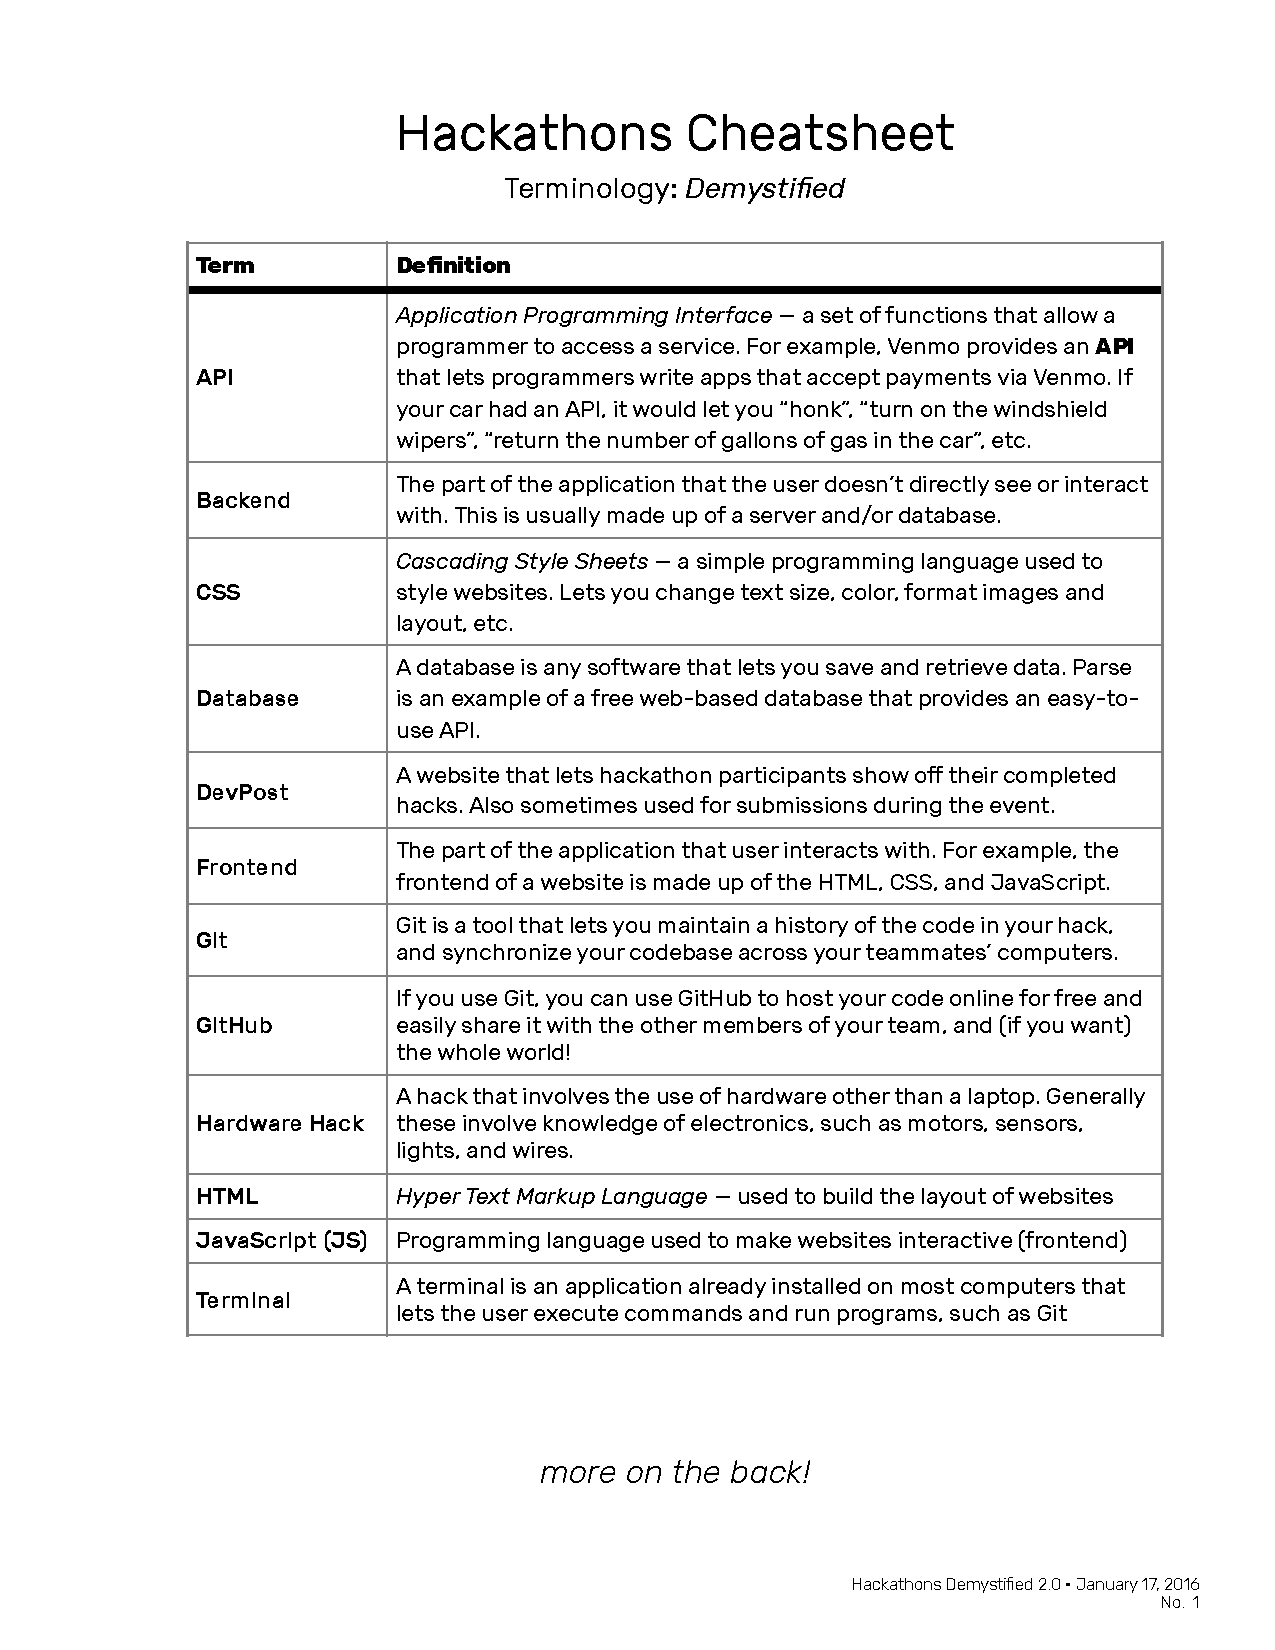
\includepdf[pages=-]{glossaryhackathonscmu.pdf}
\newpage
\section {FAQ}
Will come soon when people actually ask questions. :) 
\begin{enumerate}
\end{enumerate}
\newpage
\section{To Do}
\begin{enumerate}
\item Descriptions for Frameworks 
\item Dedicated section for commonly used git commands (and super useful ones, like push, pull, commit, commit amend, merge, cherry-pick, etc)
\item More information on marginalized groups in CS and other clubs
\item More detailed information about making websites
\end{enumerate}
\end {document}
